\subsubsection{Le concept d'équité}

Définir ce qu'est l'équité est une tâche complexe. En effet, l'équité est un concept subjectif, qui peut être mesurée avec différentes métriques. Qu'est ce qui doit peser le plus ?

Il est possible de voir l'équité sous plusieurs approches : \textcolor{red}{*équité horizontale et verticale*}

\subsubsection{L'équité entre les cyclistes}

Nous retrouvons ce problème lorsque nous essayons de définir ce qu'est un réseau cyclable équitable. Un réseau cyclable équitable permettrait à tous les usagers de se déplacer aussi facilement, quel que soit l'endroit où ils habitent, leur âge, leur niveau d'expérience, etc. 

Par exemple, on peut considérer que l'équité est atteinte lorsque tous les usagers ont accès aux mêmes infrastructures, ou lorsque les infrastructures sont adaptées aux besoins de chaque usager.

Pour un réseau cyclable, l'équité horizontale se réfère par exemple à l'égalité d'accès aux infrastructures pour tous les usagers, tandis que l'équité verticale se réfère à l'adaptation des infrastructures aux besoins de chaque usager.

Un travail de réflexion sur qu'est ce que l'équité, qu'est ce qui doit être priorisé et sur quel(s) critère(s) d'équité choisir a été réalisé par Lou-ann Deniau, en stage au département Génie de l'Aménagement et Environnement de Polytech Tours en même temps que moi. En se concertant, nous avons pu définir des critères d'équité pour l'optimisation du réseau cyclable, qui soient à la fois pertinents et réalisables informatiquement, en fonction des données présentes, des données que l'on peut croiser, de ce qui ne soit pas trop dur à programmer.

Il existe plusieurs aspects à prendre en compte pour juger de l'équité d'un réseau cyclable. On peut les regrouper en six catégories : 

% \begin{equation}\label{key}
%    \parbox{1\textwidth}{
%         \begin{itemize}
%         \item Les caractéristiques socio-démographiques
%         \item L'accès à un vélo et à une infrastructure cyclable
%         \item Les infrastructures et la cyclabilité
%         \item L'accès à un stationnement vélo et aux opportunités
%         \item Les motifs du trajet
%         \item La diversité des opportunités de destination
%     \end{itemize}
%    }
% \end{equation}

\begin{itemize} \label{categories_eq}
    \item Les caractéristiques socio-démographiques
    \item L'accès à un vélo et à une infrastructure cyclable
    \item Les infrastructures et la cyclabilité
    \item L'accès à un stationnement vélo et aux opportunités
    \item Les motifs du trajet
    \item La diversité des opportunités de destination
\end{itemize}
Elles sont présentées dans la figure \ref{fig:d1}.

\begin{figure}[h]
    \centering
    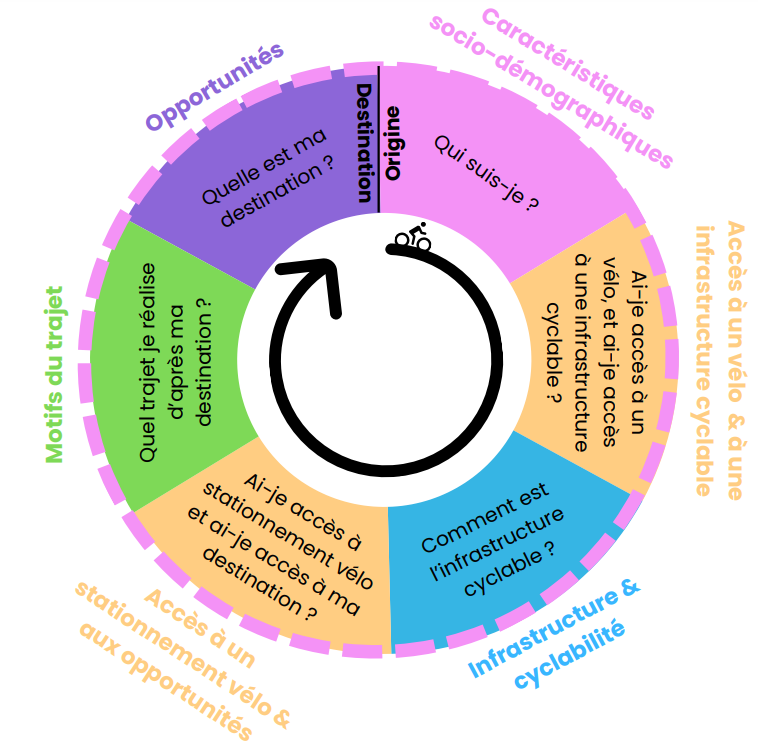
\includegraphics[width=0.5\linewidth]{deniau.png}
    \caption{Déroulé d'un trajet en vélo sous toutes ses dimensions - DENIAU, 2025}
    \label{fig:d1}
\end{figure}

